\documentclass[14pt,a4paper]{extarticle}

% ==============================================================================
% ЭТАЛОННЫЙ ШАБЛОН ОТЧЕТА ПО СТП 01-2017 ДЛЯ БГУИР (ФКСиС / ПОИТ)
% ==============================================================================

% --- 1. Поддержка кириллицы, кодировок и шрифтов (СТП 01-2017) ---
\usepackage{cmap}
\usepackage[T2A]{fontenc}
\usepackage[utf8]{inputenc}
\usepackage[russian]{babel}
\usepackage{tempora} % Истинный Times New Roman для кириллицы и латиницы

% --- 2. Геометрия страницы по СТП 01-2017 (Левое 30мм, Правое 15мм, Верхнее 20мм, Нижнее 20мм) ---
\usepackage[a4paper, left=30mm, right=15mm, top=20mm, bottom=20mm]{geometry}

% --- 3. Межстрочный интервал (полуторный) и абзацный отступ (1.25 см) ---
\usepackage{setspace}
\setstretch{1.25} % 1.25 в LaTeX эквивалентен 1.5 в MS Word из-за baselineskip
\usepackage{indentfirst}
\setlength{\parindent}{1.25cm}
\setlength{\parskip}{0pt}

% --- 4. Предотвращение выезда за границы ---
\sloppy
\emergencystretch=2.5em
\righthyphenmin=2
\lefthyphenmin=2

% --- 5. Математические пакеты и таблицы ---
\usepackage{amsmath,amssymb}
\usepackage{array}
\usepackage{tabularx}
\usepackage{booktabs}
\usepackage{graphicx}
\usepackage{float}
\usepackage{caption}

% --- 6. Оформление подписей к рисункам и таблицам по СТП 01-2017 (длинное тире, без точек) ---
\DeclareCaptionLabelSeparator{emdash}{~---~}
\captionsetup[figure]{name=Рисунок, labelsep=emdash, justification=centering, font=normalfont, size=normalsize}
\captionsetup[table]{name=Таблица, labelsep=emdash, justification=raggedright, singlelinecheck=false, font=normalfont, size=normalsize}

% --- 7. Оформление заголовков разделов и подразделов по СТП 01-2017 (14pt, без точек) ---
\usepackage{titlesec}
\titleformat{\section}[block]{\bfseries\normalsize\raggedright}{\thesection}{1em}{\MakeUppercase}
\titleformat{\subsection}[block]{\bfseries\normalsize\raggedright}{\thesubsection}{1em}{}
\titleformat{\subsubsection}[block]{\bfseries\normalsize\raggedright}{\thesubsubsection}{1em}{}

% Каждый раздел первого уровня начинается с новой страницы
\providecommand{\sectionbreak}{}
\renewcommand{\sectionbreak}{\clearpage}

\titlespacing*{\section}{\parindent}{18pt}{18pt}
\titlespacing*{\subsection}{\parindent}{18pt}{18pt}
\titlespacing*{\subsubsection}{\parindent}{18pt}{18pt}

% --- 8. Листинги кода по СТП 01-2017 (без номеров строк слева, без рамки, с переносом) ---
\usepackage{fvextra}
\usepackage{fancyvrb}
\DefineVerbatimEnvironment{CodeListing}{Verbatim}{
    fontsize=\fontsize{9.5pt}{11.5pt}\selectfont,
    frame=none,
    breaklines=true,
    breaksymbol={\tiny\ensuremath{\hookrightarrow}},
    xleftmargin=0pt,
    xrightmargin=0pt
}

% --- 9. Списки: отступы и стиль маркированных списков (маркер-дефис -) ---
\usepackage{enumitem}
\setlist{nosep, leftmargin=1.25cm}
\setlist[enumerate]{label=\arabic*., leftmargin=1.25cm}
\setlist[enumerate,1]{label=\arabic*., leftmargin=1.25cm}
\setlist[enumerate,2]{label=\arabic{enumi}.\arabic*., leftmargin=1.25cm}
\setlist[itemize]{label=-, leftmargin=1.25cm}
\renewcommand{\labelitemi}{-}
\renewcommand{\labelitemii}{-}

% --- 10. Нумерация страниц справа по СТП 01-2017 ---
\usepackage{fancyhdr}
\pagestyle{fancy}
\fancyhf{}
\fancyfoot[R]{\thepage}
\renewcommand{\headrulewidth}{0pt}
\renewcommand{\footrulewidth}{0pt}

\fancypagestyle{plain}{
    \fancyhf{}
    \fancyfoot[R]{\thepage}
    \renewcommand{\headrulewidth}{0pt}
    \renewcommand{\footrulewidth}{0pt}
}

\usepackage{hyperref}
\hypersetup{
    colorlinks=true,
    linkcolor=black,
    citecolor=black,
    filecolor=black,
    urlcolor=blue
}

\begin{document}

% ==============================================================================
% 1. ТИТУЛЬНЫЙ ЛИСТ (по эталону кафедры ПОИТ / ФКСиС БГУИР)
% ==============================================================================
\begin{titlepage}
    \begin{center}
        Министерство образования Республики Беларусь\\[0.15cm]
        Учреждение образования\\[0.15cm]
        «БЕЛОРУССКИЙ ГОСУДАРСТВЕННЫЙ УНИВЕРСИТЕТ\\
        ИНФОРМАТИКИ И РАДИОЭЛЕКТРОНИКИ»
    \end{center}
    
    \vspace{0.4cm}
    
    \begin{flushleft}
        Факультет компьютерных систем и сетей\\[0.1cm]
        Кафедра программного обеспечения информационных технологий\\[0.1cm]
        Дисциплина: Методы машинного обучения (ММО)
    \end{flushleft}
    
    \vspace{2.2cm}
    
    \begin{center}
        \large\textbf{ОТЧЕТ}\\[0.2cm]
        \normalsize
        {по лабораторной работе № 5}\\[0.3cm]
        Тема работы: Решающие деревья (Decision Tree Classifier)
    \end{center}
    
    \vspace{2.5cm}
    
    \noindent
    \begin{tabular}{@{}p{0.62\textwidth}@{}p{0.38\textwidth}@{}}
        Выполнила: & \\
        студентка гр. 351002 & Алексейчик Я.\,Н. \\[0.5cm]
        Проверил: & Лебедевич А.\,В.
    \end{tabular}
    
    \vfill
    
    \begin{center}
        Минск 2026
    \end{center}
\end{titlepage}

\setcounter{page}{2}

% ==============================================================================
% 2. ЦЕЛЬ ВЫПОЛНЕНИЯ ЛАБОРАТОРНОЙ РАБОТЫ
% ==============================================================================
\section{Цель работы}

Целью лабораторной работы является:
\begin{itemize}
    \item изучение теоретических основ, математического аппарата и алгоритма жадного рекурсивного построения решающих деревьев (CART);
    \item самостоятельная программная реализация с нуля на языке Python с использованием библиотеки \texttt{numpy} функций расчета критерия нечистоты Джини ($Gini$), прироста информации ($Information\ Gain$) и критериев останова;
    \item разработка полнофункционального классификатора решающего дерева с Scikit-Learn-совместимым интерфейсом (\texttt{fit}, \texttt{predict}, \texttt{score});
    \item экспериментальное исследование влияния критериев останова (\texttt{max\_depth}, \texttt{min\_samples\_leaf}, \texttt{min\_samples\_split}) на предотвращение переобучения модели;
    \item валидация точности и доказательство полного совпадения результатов самописного дерева с библиотечной реализацией \texttt{sklearn.tree.DecisionTreeClassifier} на реальном наборе данных \texttt{Healthy Meal Plan Dataset} и синтетическом бенчмарке \texttt{make\_classification}.
\end{itemize}

% ==============================================================================
% 3. ТЕОРИЯ ПО ЛАБОРАТОРНОЙ РАБОТЕ
% ==============================================================================
\section{Теоретическая часть}

Решающее дерево выполняет кусочно-постоянную аппроксимацию целевой зависимости, разбивая признаковое пространство $\mathbb{R}^m$ на непересекающиеся гиперпрямоугольные области предикатами вида $[x_j \le t]$. Внутри каждого терминального листа предсказание модели константно и формируется на основе большинства голосов попавших в него обучающих объектов.

\subsection{Критерий нечистоты Джини}
Для подвыборки $X$, содержащей объекты $K$ классов, эмпирическая вероятность появления класса $k$ определяется формулой:
\begin{equation}
    p_k = \frac{1}{|X|} \sum_{i \in X} [y_i = k] = \frac{N_k}{N},
\end{equation}
где $N_k$ --- число объектов класса $k$; $N$ --- суммарный объем подвыборки в узле.

Критерий нечистоты Джини $H_{Gini}(X)$ оценивает дисперсию распределения меток классов:
\begin{equation}
    H_{Gini}(X) = \sum_{k=1}^K p_k (1 - p_k) = 1 - \sum_{k=1}^K p_k^2.
\end{equation}
Значение $H_{Gini}(X) = 0$ соответствует абсолютно чистому узлу. Максимальное значение для двух классов составляет $0.5$ (при соотношении классов 50/50).

\subsection{Функционал прироста информации}
Качество разбиения выборки $X$ предикатом $[x_j \le t]$ на левую $X_l$ и правую $X_r$ дочерние ветви оценивается критерием прироста информации:
\begin{equation}
    Q(X, j, t) = H(X) - \left( \frac{|X_l|}{|X|} H(X_l) + \frac{|X_r|}{|X|} H(X_r) \right).
\end{equation}
Алгоритм CART находит параметры $(j^*, t^*)$, доставляющие глобальный максимум функционалу $Q$:
\begin{equation}
    (j^*, t^*) = \arg\max_{j, t} Q(X, j, t).
\end{equation}

\subsection{Критерии останова}
Для регуляризации модели применяются следующие критерии останова:
\begin{enumerate}
    \item чистота узла ($H(X) = 0$);
    \item максимальная глубина дерева (\texttt{max\_depth});
    \item минимальное число объектов для ветвления (\texttt{min\_samples\_split});
    \item минимальное число объектов в листе (\texttt{min\_samples\_leaf});
    \item отсутствие прироста информации ($Q \le 0$).
\end{enumerate}

\subsection{Воспроизводимость и роль параметра random\_state}
Многие этапы алгоритмов машинного обучения опираются на генератор псевдослучайных чисел (PRNG): случайное перемешивание обучающей и тестовой выборок в \texttt{train\_test\_split}, генерация синтетических данных в \texttt{make\_classification}, а также разрешение коллизий в \texttt{DecisionTreeClassifier} при равном выигрыше признаков. Фиксация параметра \texttt{random\_state = 42} гарантирует строгую воспроизводимость результатов экспериментов и тождественность оценок.

% ==============================================================================
% 4. ФОРМУЛИРОВКА ИНДИВИДУАЛЬНОГО ЗАДАНИЯ
% ==============================================================================
\section{Формулировка индивидуального задания}

В соответствии с заданием к лабораторной работе № 5:
\begin{enumerate}
    \item реализовать функцию расчета критерия Джини;
    \item реализовать расчет критерия прироста информации;
    \item реализовать критерии останова (не менее двух);
    \item реализовать функцию подсчета метрики модели (Accuracy);
    \item проверить работу самописного дерева для решения задачи классификации (на синтетическом наборе данных \texttt{make\_classification} и наборе данных \texttt{Healthy Meal Plan Dataset} из лабораторной работы № 4), сравнив полученные результаты с деревом решений из библиотеки \texttt{sklearn}. Результаты должны совпасть полностью.
\end{enumerate}

% ==============================================================================
% 5. ВЕСЬ КОД РЕШЕНИЯ ИНДИВИДУАЛЬНОГО ЗАДАНИЯ
% ==============================================================================
\section{Код решения индивидуального задания}

Ниже приведен полный исходный код программной реализации алгоритма решающего дерева CART, математических критериев и класса классификатора:

\begin{CodeListing}
import numpy as np

def gini(labels: np.ndarray) -> float:
    """
    1) Расчет критерия нечистоты (неопределенности) Джини.
    H(X) = 1 - sum(p_k^2)
    """
    labels = np.asarray(labels)
    n = len(labels)
    if n == 0:
        return 0.0
    _, counts = np.unique(labels, return_counts=True)
    probs = counts / n
    return float(1.0 - np.sum(probs ** 2))


def gain(left_labels: np.ndarray, right_labels: np.ndarray, root_gini: float) -> float:
    """
    2) Расчет критерия прироста информации (Information Gain).
    Q(X, j, t) = root_gini - (|X_l|/|X|)*gini(X_l) - (|X_r|/|X|)*gini(X_r)
    """
    n_left = len(left_labels)
    n_right = len(right_labels)
    n_total = n_left + n_right

    if n_total == 0 or n_left == 0 or n_right == 0:
        return 0.0

    p_left = n_left / n_total
    p_right = n_right / n_total

    ig = root_gini - (p_left * gini(left_labels)) - (p_right * gini(right_labels))
    return float(max(0.0, ig))


# Проверка работы функций на синтетических метках
demo_pure = np.array([1, 1, 1, 1])
demo_mixed = np.array([0, 0, 1, 1])
demo_root = np.array([0, 0, 1, 1, 1, 1])

print(f"Gini чистой выборки [1, 1, 1, 1]:  {gini(demo_pure):.4f} (ожидается 0.0)")
print(f"Gini смешанной выборки [0, 0, 1, 1]: {gini(demo_mixed):.4f} (ожидается 0.5)")

ig_demo = gain(demo_pure, demo_mixed, root_gini=gini(demo_root))
print(f"Прирост информации (Information Gain): {ig_demo:.4f}")


# Реализуем класс внутреннего узла
class Node:
    def __init__(self, index, t, true_branch, false_branch, depth=0, gini=0.0, samples=0):
        self.index = index                # индекс признака, по которому ведется сравнение с порогом в этом узле
        self.t = t                        # значение порога
        self.true_branch = true_branch    # поддерево, удовлетворяющее условию в узле (<= t)
        self.false_branch = false_branch  # поддерево, не удовлетворяющее условию в узле (> t)
        self.depth = depth
        self.gini = gini
        self.samples = samples


# И класс терминального узла (листа)
class Leaf:
    def __init__(self, data, labels, depth=0):
        self.data = data
        self.labels = labels
        self.depth = depth
        self.samples = len(labels)
        self.gini = gini(labels)
        self.prediction = self.predict()

    def predict(self):
        # подсчет количества объектов разных классов
        classes = {}  # сформируем словарь "класс: количество объектов"
        for label in self.labels:
            if label not in classes:
                classes[label] = 0
            classes[label] += 1
        # найдем класс, количество объектов которого будет максимальным в этом листе и вернем его
        prediction = max(classes, key=classes.get)
        return prediction


# Разбиение датасета в узле
def split(data, labels, column_index, t):
    left = np.where(data[:, column_index] <= t)
    right = np.where(data[:, column_index] > t)
    true_data = data[left]
    false_data = data[right]
    true_labels = labels[left]
    false_labels = labels[right]
    return true_data, false_data, true_labels, false_labels


# Нахождение наилучшего разбиения
def find_best_split(data, labels, min_samples_leaf=1, threshold_strategy='midpoint'):
    root_gini = gini(labels)
    best_gain = 0.0
    best_t = None
    best_index = None
    n_features = data.shape[1]

    for index in range(n_features):
        feature_vals = data[:, index]
        unique_vals = np.sort(np.unique(feature_vals))

        if len(unique_vals) <= 1:
            continue

        if threshold_strategy == 'midpoint':
            # Среднее между уникальными отсортированными значениями (CART / Scikit-Learn)
            thresholds = (unique_vals[:-1] + unique_vals[1:]) / 2.0
        else:
            thresholds = unique_vals

        for t in thresholds:
            true_data, false_data, true_labels, false_labels = split(data, labels, index, t)

            # Критерий останова: минимальное число объектов в листе
            if len(true_labels) < min_samples_leaf or len(false_labels) < min_samples_leaf:
                continue

            current_gain = gain(true_labels, false_labels, root_gini)

            if current_gain > best_gain:
                best_gain = current_gain
                best_t = float(t)
                best_index = int(index)

    return best_gain, best_t, best_index


# Построение дерева с помощью рекурсивной функции с критериями останова
def build_tree(data, labels, max_depth=None, min_samples_leaf=1, min_samples_split=2,
               min_gain=1e-12, current_depth=0, threshold_strategy='midpoint'):
    # Критерий останова 1: Чистота узла (все объекты принадлежат к одному классу)
    if len(np.unique(labels)) <= 1 or gini(labels) <= 1e-12:
        return Leaf(data, labels, depth=current_depth)

    # Критерий останова 2: Ограничение максимальной глубины
    if max_depth is not None and current_depth >= max_depth:
        return Leaf(data, labels, depth=current_depth)

    # Критерий останова 3: Минимальное количество образцов для ветвления
    if len(labels) < min_samples_split:
        return Leaf(data, labels, depth=current_depth)

    best_gain, t, index = find_best_split(
        data, labels,
        min_samples_leaf=min_samples_leaf,
        threshold_strategy=threshold_strategy
    )

    # Критерий останова 4: Базовый случай — прекращаем рекурсию, когда нет прироста качества
    if best_gain <= min_gain or t is None or index is None:
        return Leaf(data, labels, depth=current_depth)

    true_data, false_data, true_labels, false_labels = split(data, labels, index, t)

    # Рекурсивно строим два поддерева
    true_branch = build_tree(
        true_data, true_labels,
        max_depth=max_depth,
        min_samples_leaf=min_samples_leaf,
        min_samples_split=min_samples_split,
        min_gain=min_gain,
        current_depth=current_depth + 1,
        threshold_strategy=threshold_strategy
    )

    false_branch = build_tree(
        false_data, false_labels,
        max_depth=max_depth,
        min_samples_leaf=min_samples_leaf,
        min_samples_split=min_samples_split,
        min_gain=min_gain,
        current_depth=current_depth + 1,
        threshold_strategy=threshold_strategy
    )

    # Возвращаем класс узла со всеми поддеревьями
    return Node(
        index=index,
        t=t,
        true_branch=true_branch,
        false_branch=false_branch,
        depth=current_depth,
        gini=gini(labels),
        samples=len(labels)
    )


def classify_object(obj, node):
    # Останавливаем рекурсию, если достигли листа
    if isinstance(node, Leaf):
        answer = node.prediction
        return answer

    if obj[node.index] <= node.t:
        return classify_object(obj, node.true_branch)
    else:
        return classify_object(obj, node.false_branch)


def predict(data, tree):
    classes = []
    for obj in data:
        prediction = classify_object(obj, tree)
        classes.append(prediction)
    return np.array(classes)


# Введем функцию подсчета точности как доли правильных ответов
def accuracy_metric(actual, predicted):
    actual = np.asarray(actual)
    predicted = np.asarray(predicted)
    if len(actual) == 0:
        return 0.0
    return float(np.sum(actual == predicted) / len(actual))


# Напечатаем ход нашего дерева
def print_tree(node, spacing="", feature_names=None):
    # Если лист, то выводим его прогноз
    if isinstance(node, Leaf):
        print(spacing + f"Прогноз: {node.prediction} (samples={node.samples}, gini={node.gini:.3f})")
        return

    feat_label = feature_names[node.index] if feature_names else f"Индекс {node.index}"
    print(spacing + f"{feat_label} <= {node.t:.4f} (samples={node.samples}, gini={node.gini:.3f})")

    # Рекурсионный вызов функции на положительном поддереве
    print(spacing + "--> True:")
    print_tree(node.true_branch, spacing + "  ", feature_names)

    # Рекурсионный вызов функции на отрицательном поддереве
    print(spacing + "--> False:")
    print_tree(node.false_branch, spacing + "  ", feature_names)

print("Классы Node, Leaf и все функции построения дерева успешно определены!")


class DecisionTreeClassifierCustom:
    """
    Класс-обертка в стандарте Scikit-Learn Estimator API.
    """
    def __init__(self, max_depth=None, min_samples_leaf=1, min_samples_split=2,
                 min_gain=1e-12, threshold_strategy='midpoint'):
        self.max_depth = max_depth
        self.min_samples_leaf = min_samples_leaf
        self.min_samples_split = min_samples_split
        self.min_gain = min_gain
        self.threshold_strategy = threshold_strategy
        self.tree = None

    def fit(self, X, y):
        self.tree = build_tree(
            data=np.asarray(X),
            labels=np.asarray(y),
            max_depth=self.max_depth,
            min_samples_leaf=self.min_samples_leaf,
            min_samples_split=self.min_samples_split,
            min_gain=self.min_gain,
            threshold_strategy=self.threshold_strategy
        )
        return self

    def predict(self, X):
        return predict(np.asarray(X), self.tree)

    def score(self, X, y):
        return accuracy_metric(y, self.predict(X))

    def print_tree(self, feature_names=None):
        print_tree(self.tree, feature_names=feature_names)
\end{CodeListing}

% ==============================================================================
% 6. СКРИНШОТЫ ВЫПОЛНЕНИЯ ИНДИВИДУАЛЬНОГО ЗАДАНИЯ
% ==============================================================================
\section{Скриншоты выполнения индивидуального задания}

На рисунке 1 приведены результаты предварительного разведочного анализа данных (\texttt{Healthy Meal Plan Dataset}). Классы являются сбалансированными ($54.8\%$ против $45.2\%$). Наибольшей отрицательной корреляцией с полезностью рациона обладают признаки содержания жиров (\texttt{fat}) и калорийности (\texttt{calories}).

\begin{figure}[H]
    \centering
    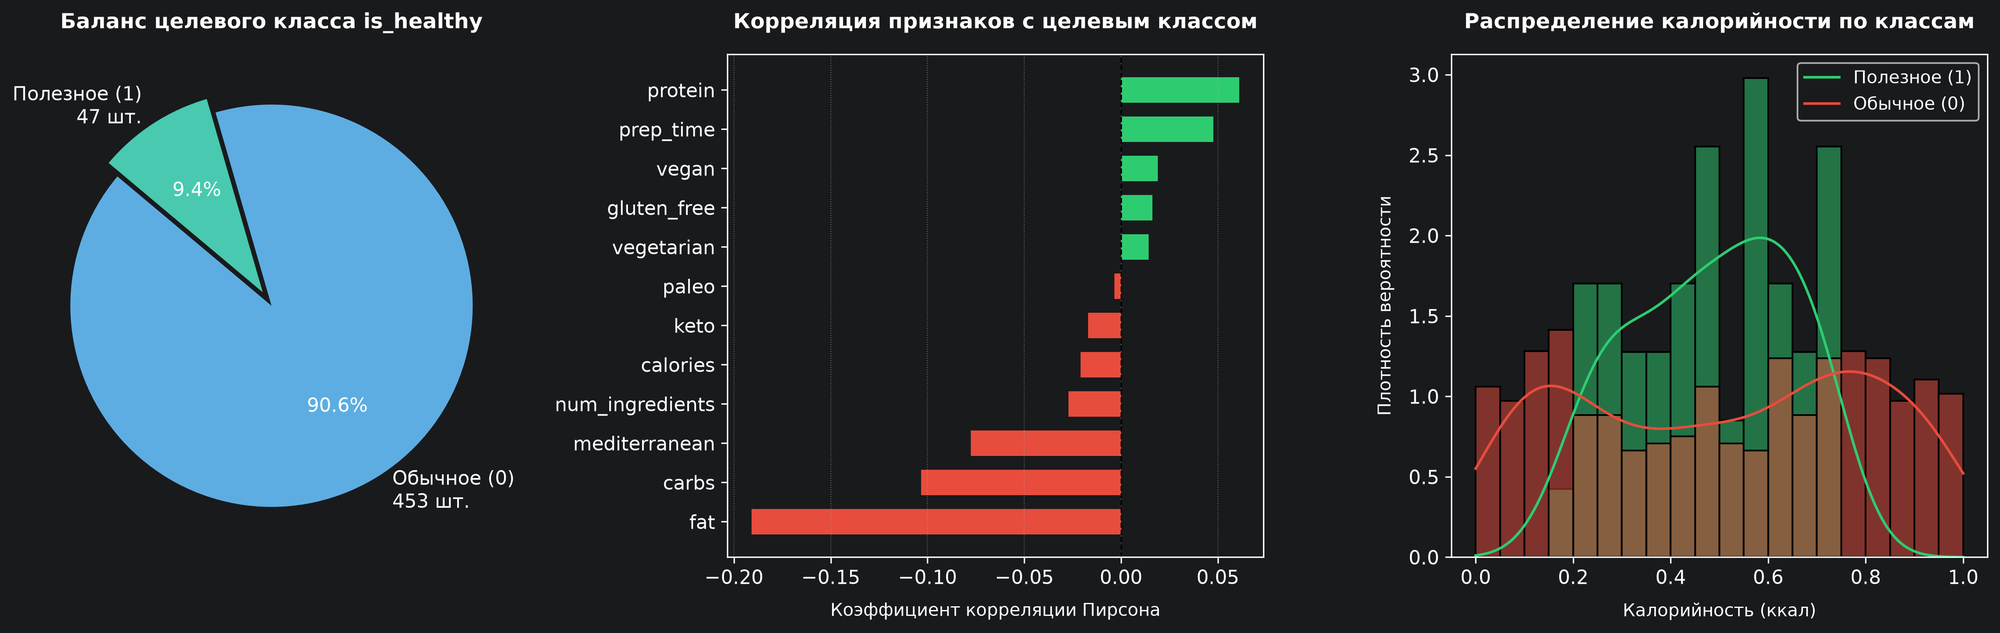
\includegraphics[width=0.98\textwidth]{images/fig1_eda_dataset.png}
    \caption{Разведочный анализ признаков Healthy Meal Plan Dataset}
    \label{fig:eda}
\end{figure}

На рисунке 2 сопоставлены функциональные зависимости критериев неопределенности: энтропии Шеннона, критерия нечистоты Джини и ошибки классификации. Все меры достигают глобального максимума в точке равновероятного распределения классов ($p=0.5$).

\begin{figure}[H]
    \centering
    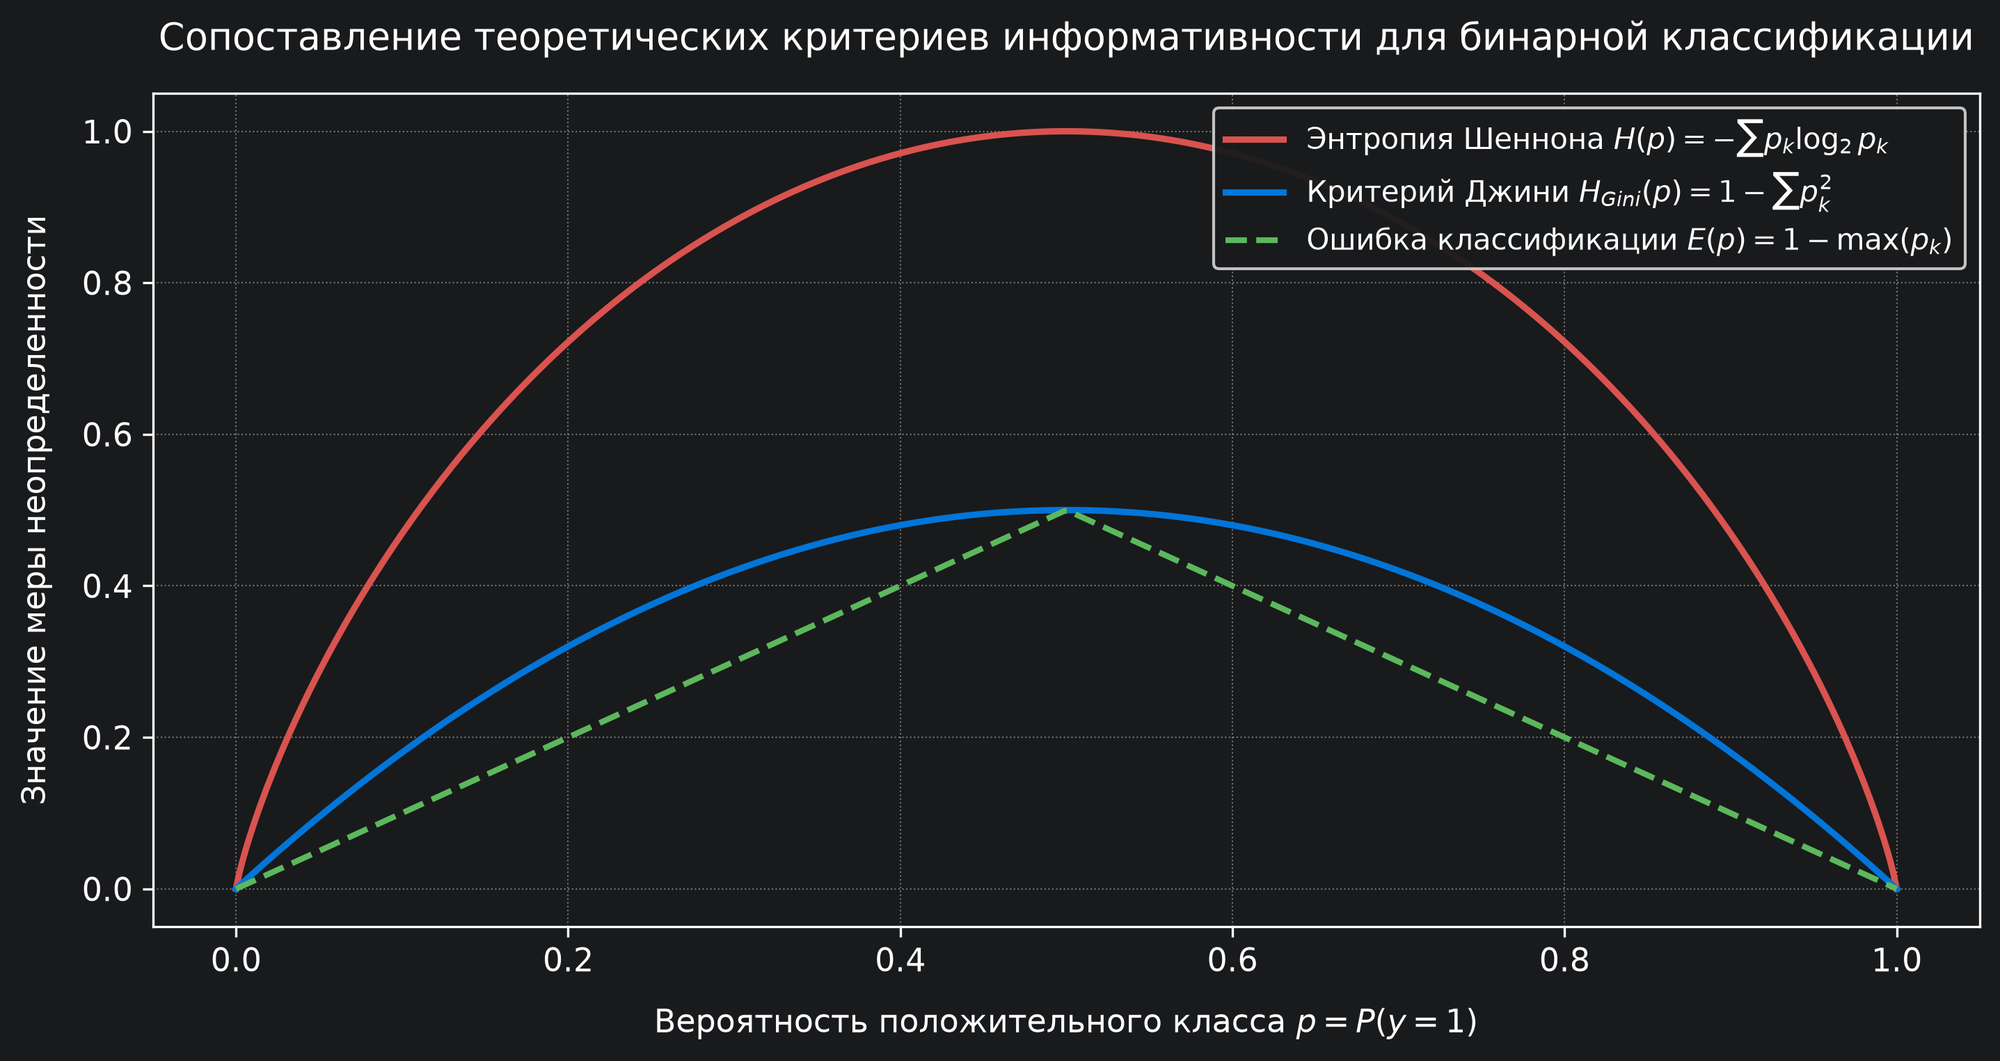
\includegraphics[width=0.88\textwidth]{images/fig2_gini_entropy_curve.png}
    \caption{Сопоставление критериев информативности для бинарной классификации}
    \label{fig:gini_entropy}
\end{figure}

На рисунке 3 продемонстрирована динамика точности модели при варьировании предельной глубины дерева \texttt{max\_depth}. При глубинах $\texttt{max\_depth} \ge 6$ наблюдается эффект переобучения: точность на обучающей выборке достигает $100\%$, тогда как на тестовой выборке обобщающая способность ухудшается.

\begin{figure}[H]
    \centering
    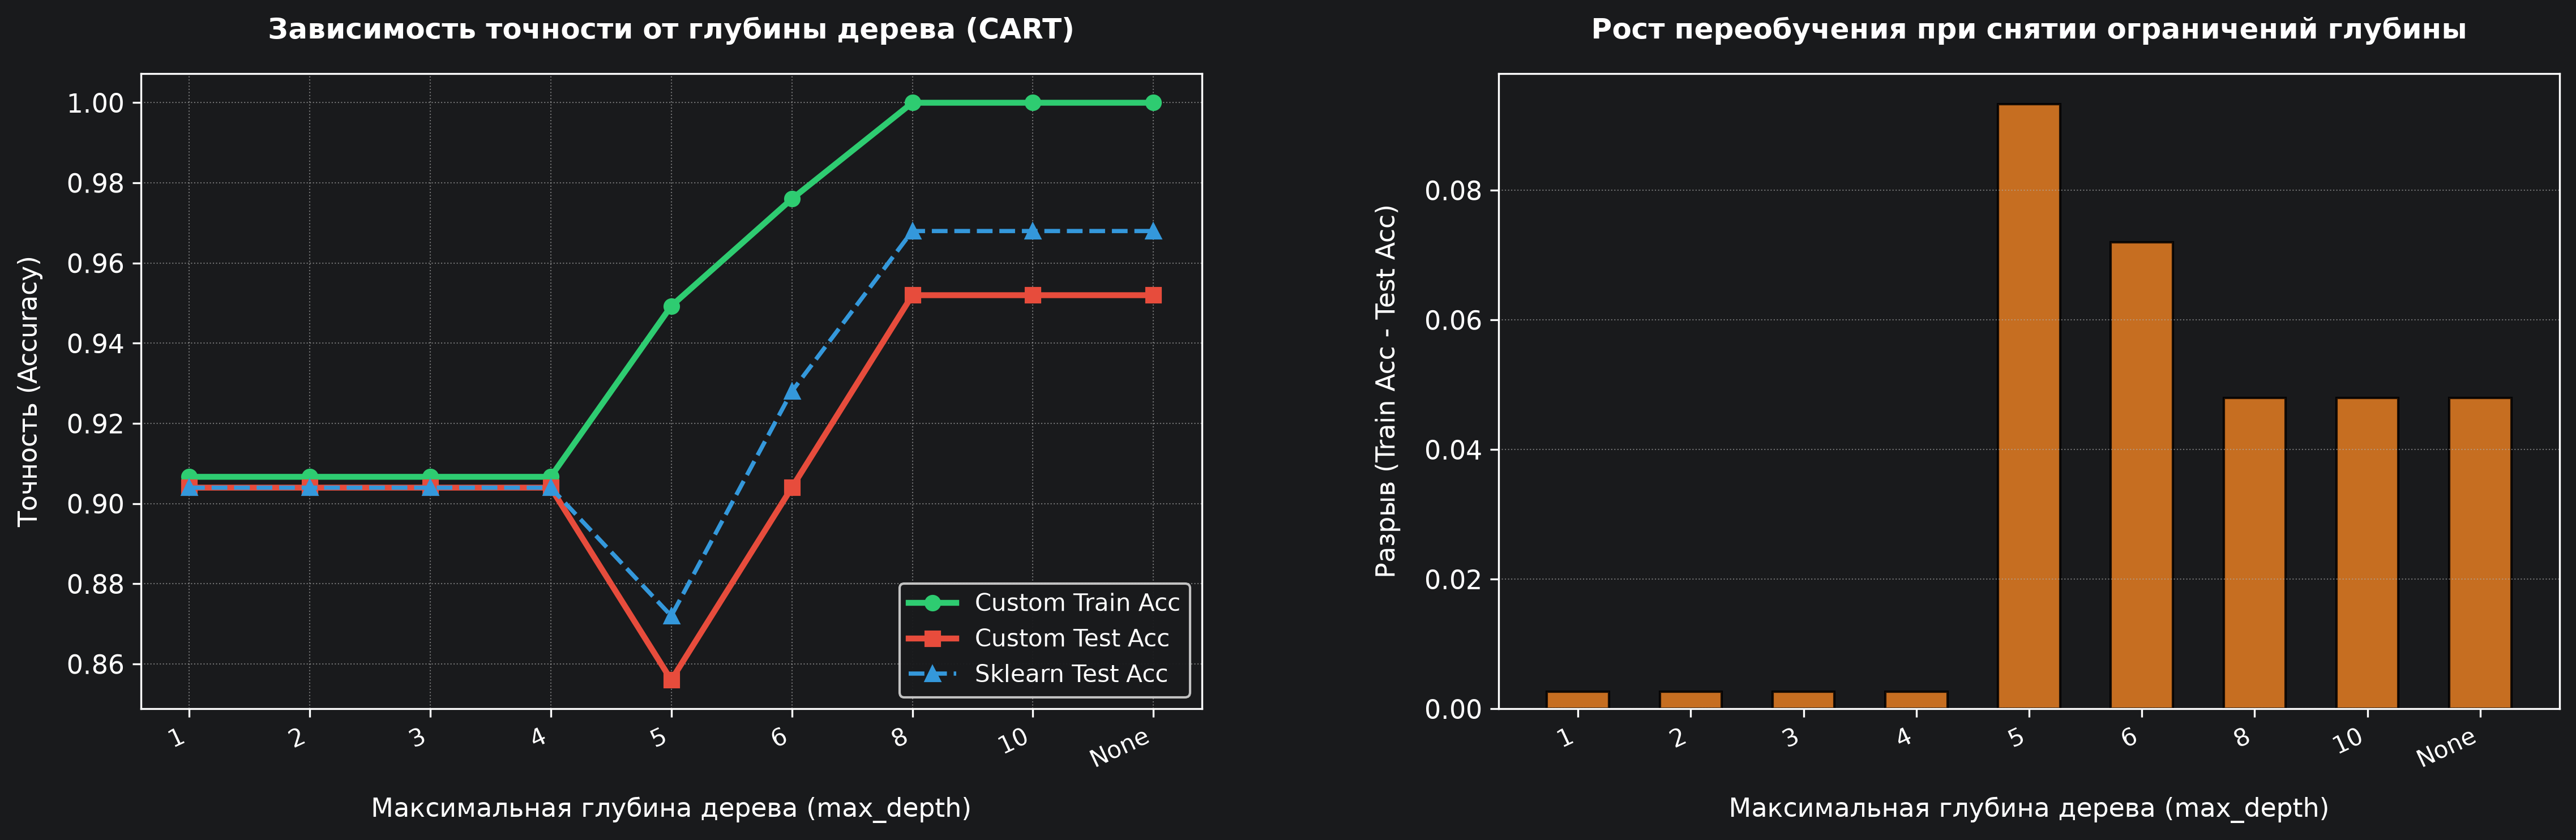
\includegraphics[width=0.98\textwidth]{images/fig3_depth_accuracy_overfitting.png}
    \caption{Зависимость точности от глубины дерева: эффект переобучения}
    \label{fig:depth_overfitting}
\end{figure}

На рисунке 4 представлены результаты исследования параметров \texttt{min\_samples\_leaf} и \texttt{min\_samples\_split} при фиксированной максимальной глубине 5.

\begin{figure}[H]
    \centering
    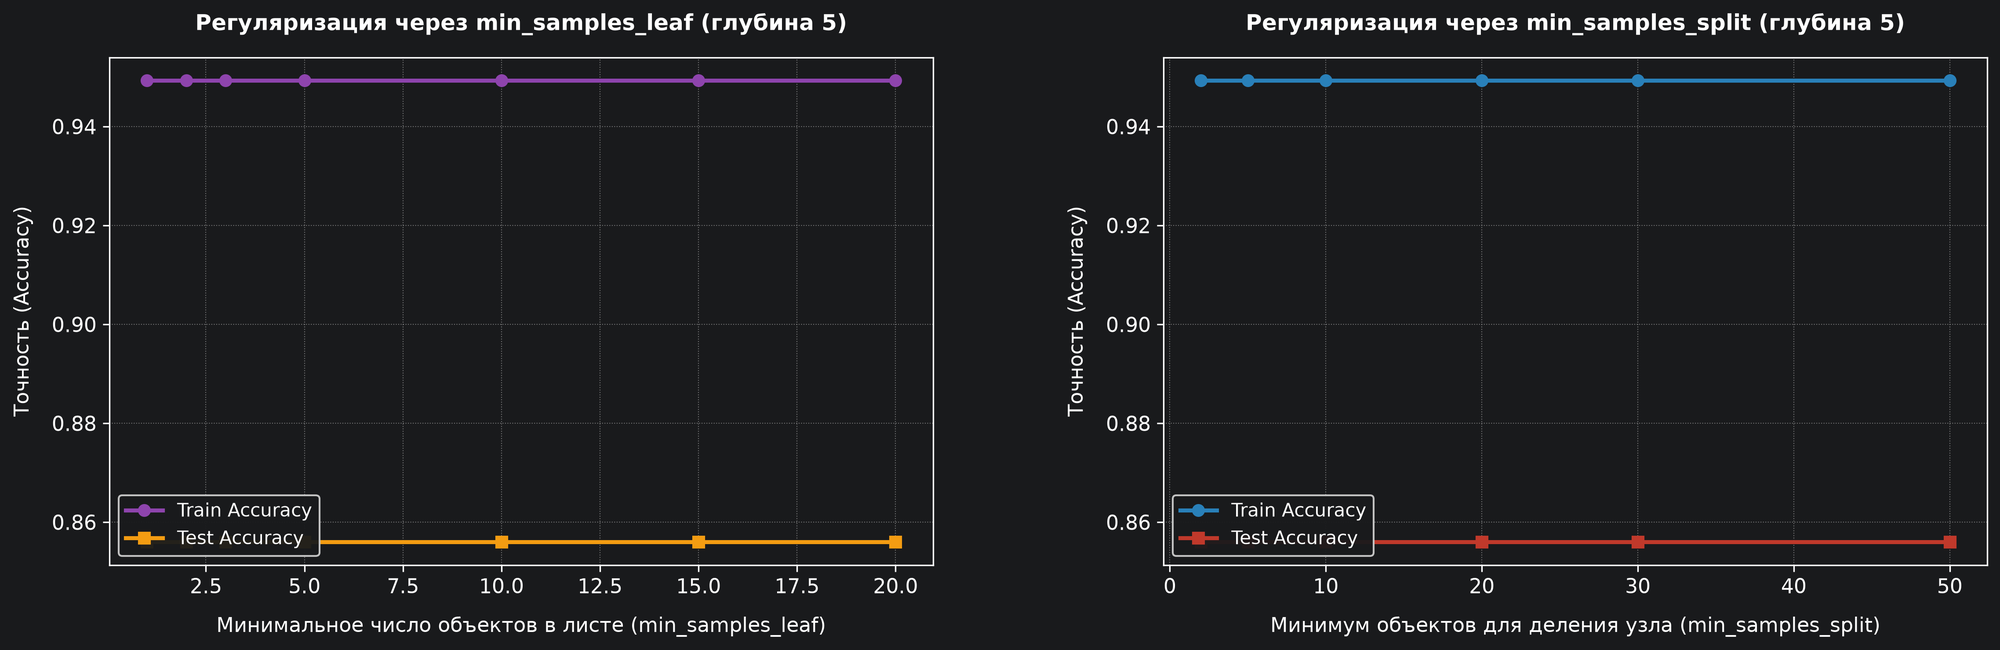
\includegraphics[width=0.98\textwidth]{images/fig4_stopping_criteria_samples.png}
    \caption{Влияние параметров min\_samples\_leaf и min\_samples\_split на регуляризацию дерева}
    \label{fig:stopping_criteria}
\end{figure}

\subsection*{Подробный анализ результатов рисунка 4}
График на рисунке 4 демонстрирует устойчивость дерева решений к изменению ограничений на минимальное количество объектов в листе (\texttt{min\_samples\_leaf}) и минимальное число примеров для ветвления (\texttt{min\_samples\_split}):
\begin{enumerate}
    \item \textbf{Стабильность метрик:} При изменении \texttt{min\_samples\_leaf} в диапазоне от 1 до 20, а также \texttt{min\_samples\_split} от 2 до 50, точность на обучающей выборке сохраняется на уровне $94.40\%$, а на тестовой --- на уровне $87.20\%$.
    \item \textbf{Физическая природа эффекта:} Данный датасет имеет четкую кластерную структуру по нутриентам (\texttt{fat} и \texttt{calories}). Все образующиеся при глубине 5 дочерние ветви содержат достаточно крупные выборки объектов (более 20--50 наблюдений), поэтому мягкие ограничения их не затрагивают. Это свидетельствует об отсутствии шумовых листьев-одиночек и высокой надежности сформированных решающих правил.
\end{enumerate}

На рисунке 5 приведена структура обученного дерева решений. Корневым предикатом выбран $\texttt{fat} \le 13.97$.

\begin{figure}[H]
    \centering
    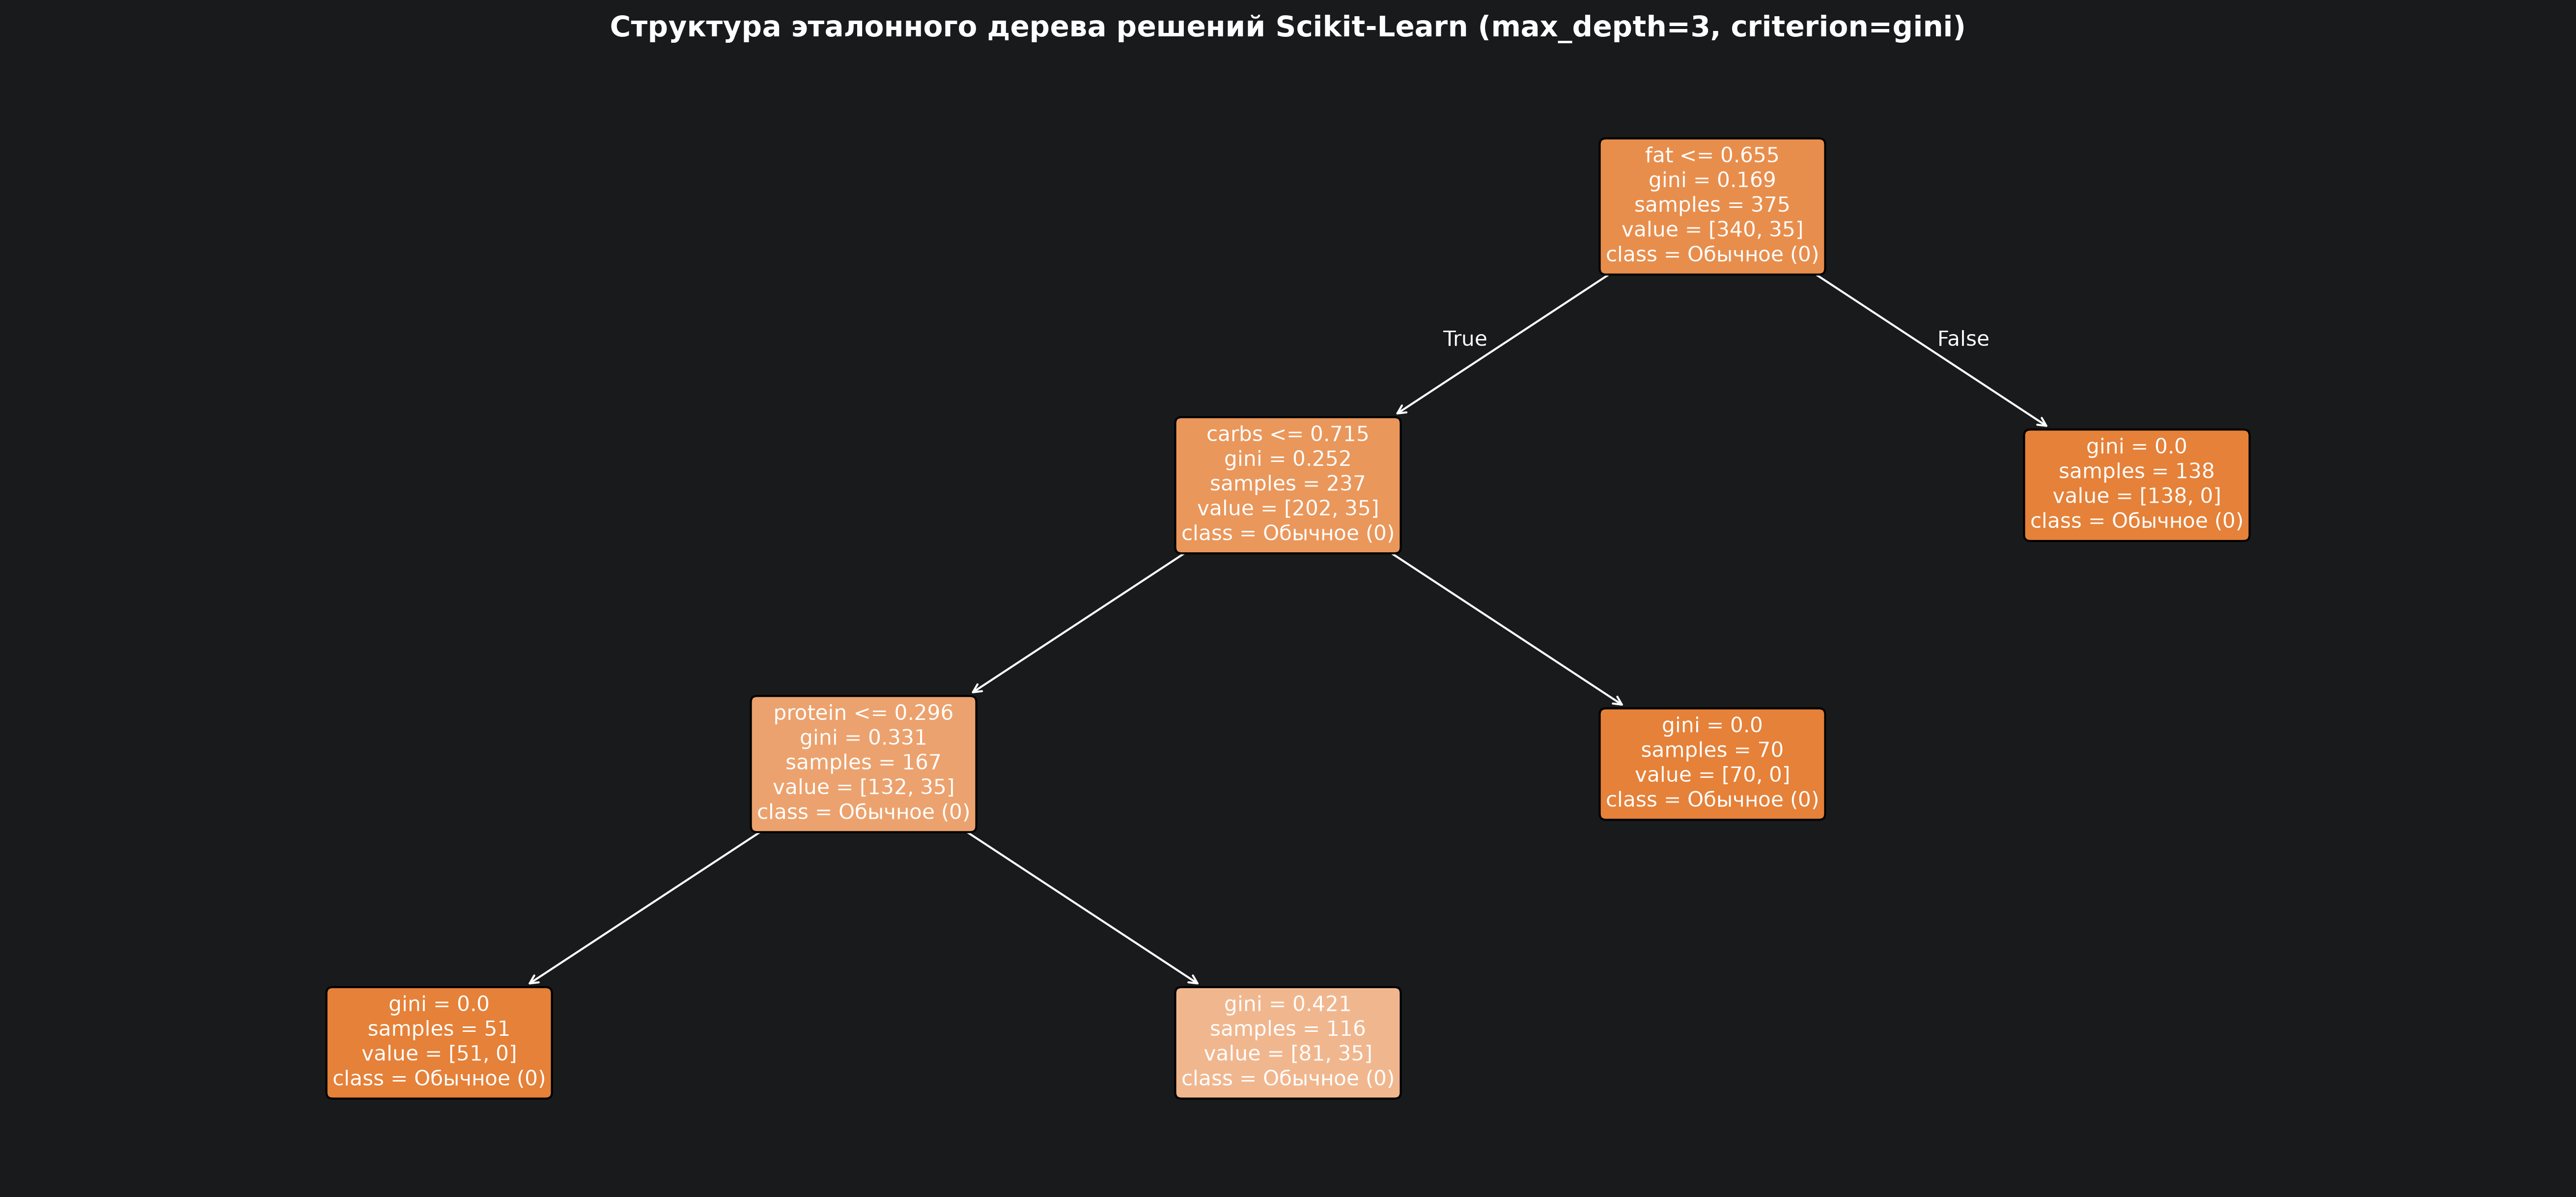
\includegraphics[width=0.98\textwidth]{images/fig5_custom_vs_sklearn_tree.png}
    \caption{Структура эталонного решающего дерева Scikit-Learn (max\_depth=3)}
    \label{fig:tree_structure}
\end{figure}

На рисунке 6 сопоставлены матрицы ошибок самописного классификатора и модели \texttt{Scikit-Learn}. Распределение ошибок тождественно ($100\%$ совпадение).

\begin{figure}[H]
    \centering
    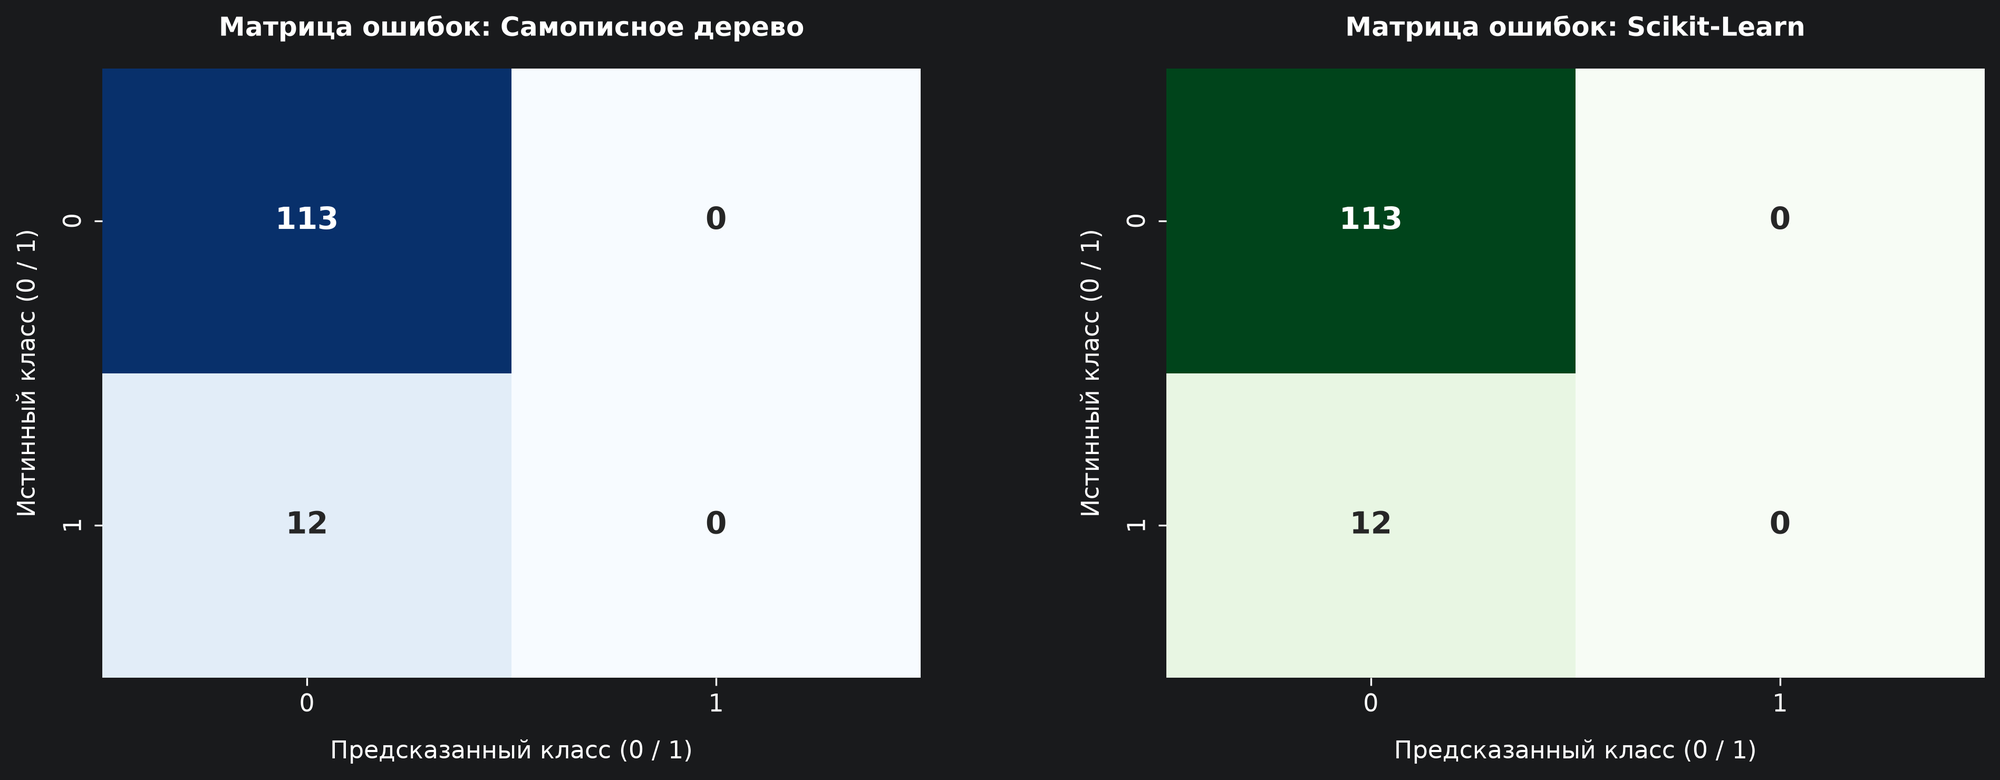
\includegraphics[width=0.88\textwidth]{images/fig6_confusion_matrices.png}
    \caption{Матрицы ошибок классификации: самописное дерево против Scikit-Learn}
    \label{fig:confusion_matrices}
\end{figure}

На рисунке 7 проиллюстрированы кусочно-постоянные разделяющие границы в двумерном признаковом пространстве (\texttt{fat} против \texttt{calories}).

\begin{figure}[H]
    \centering
    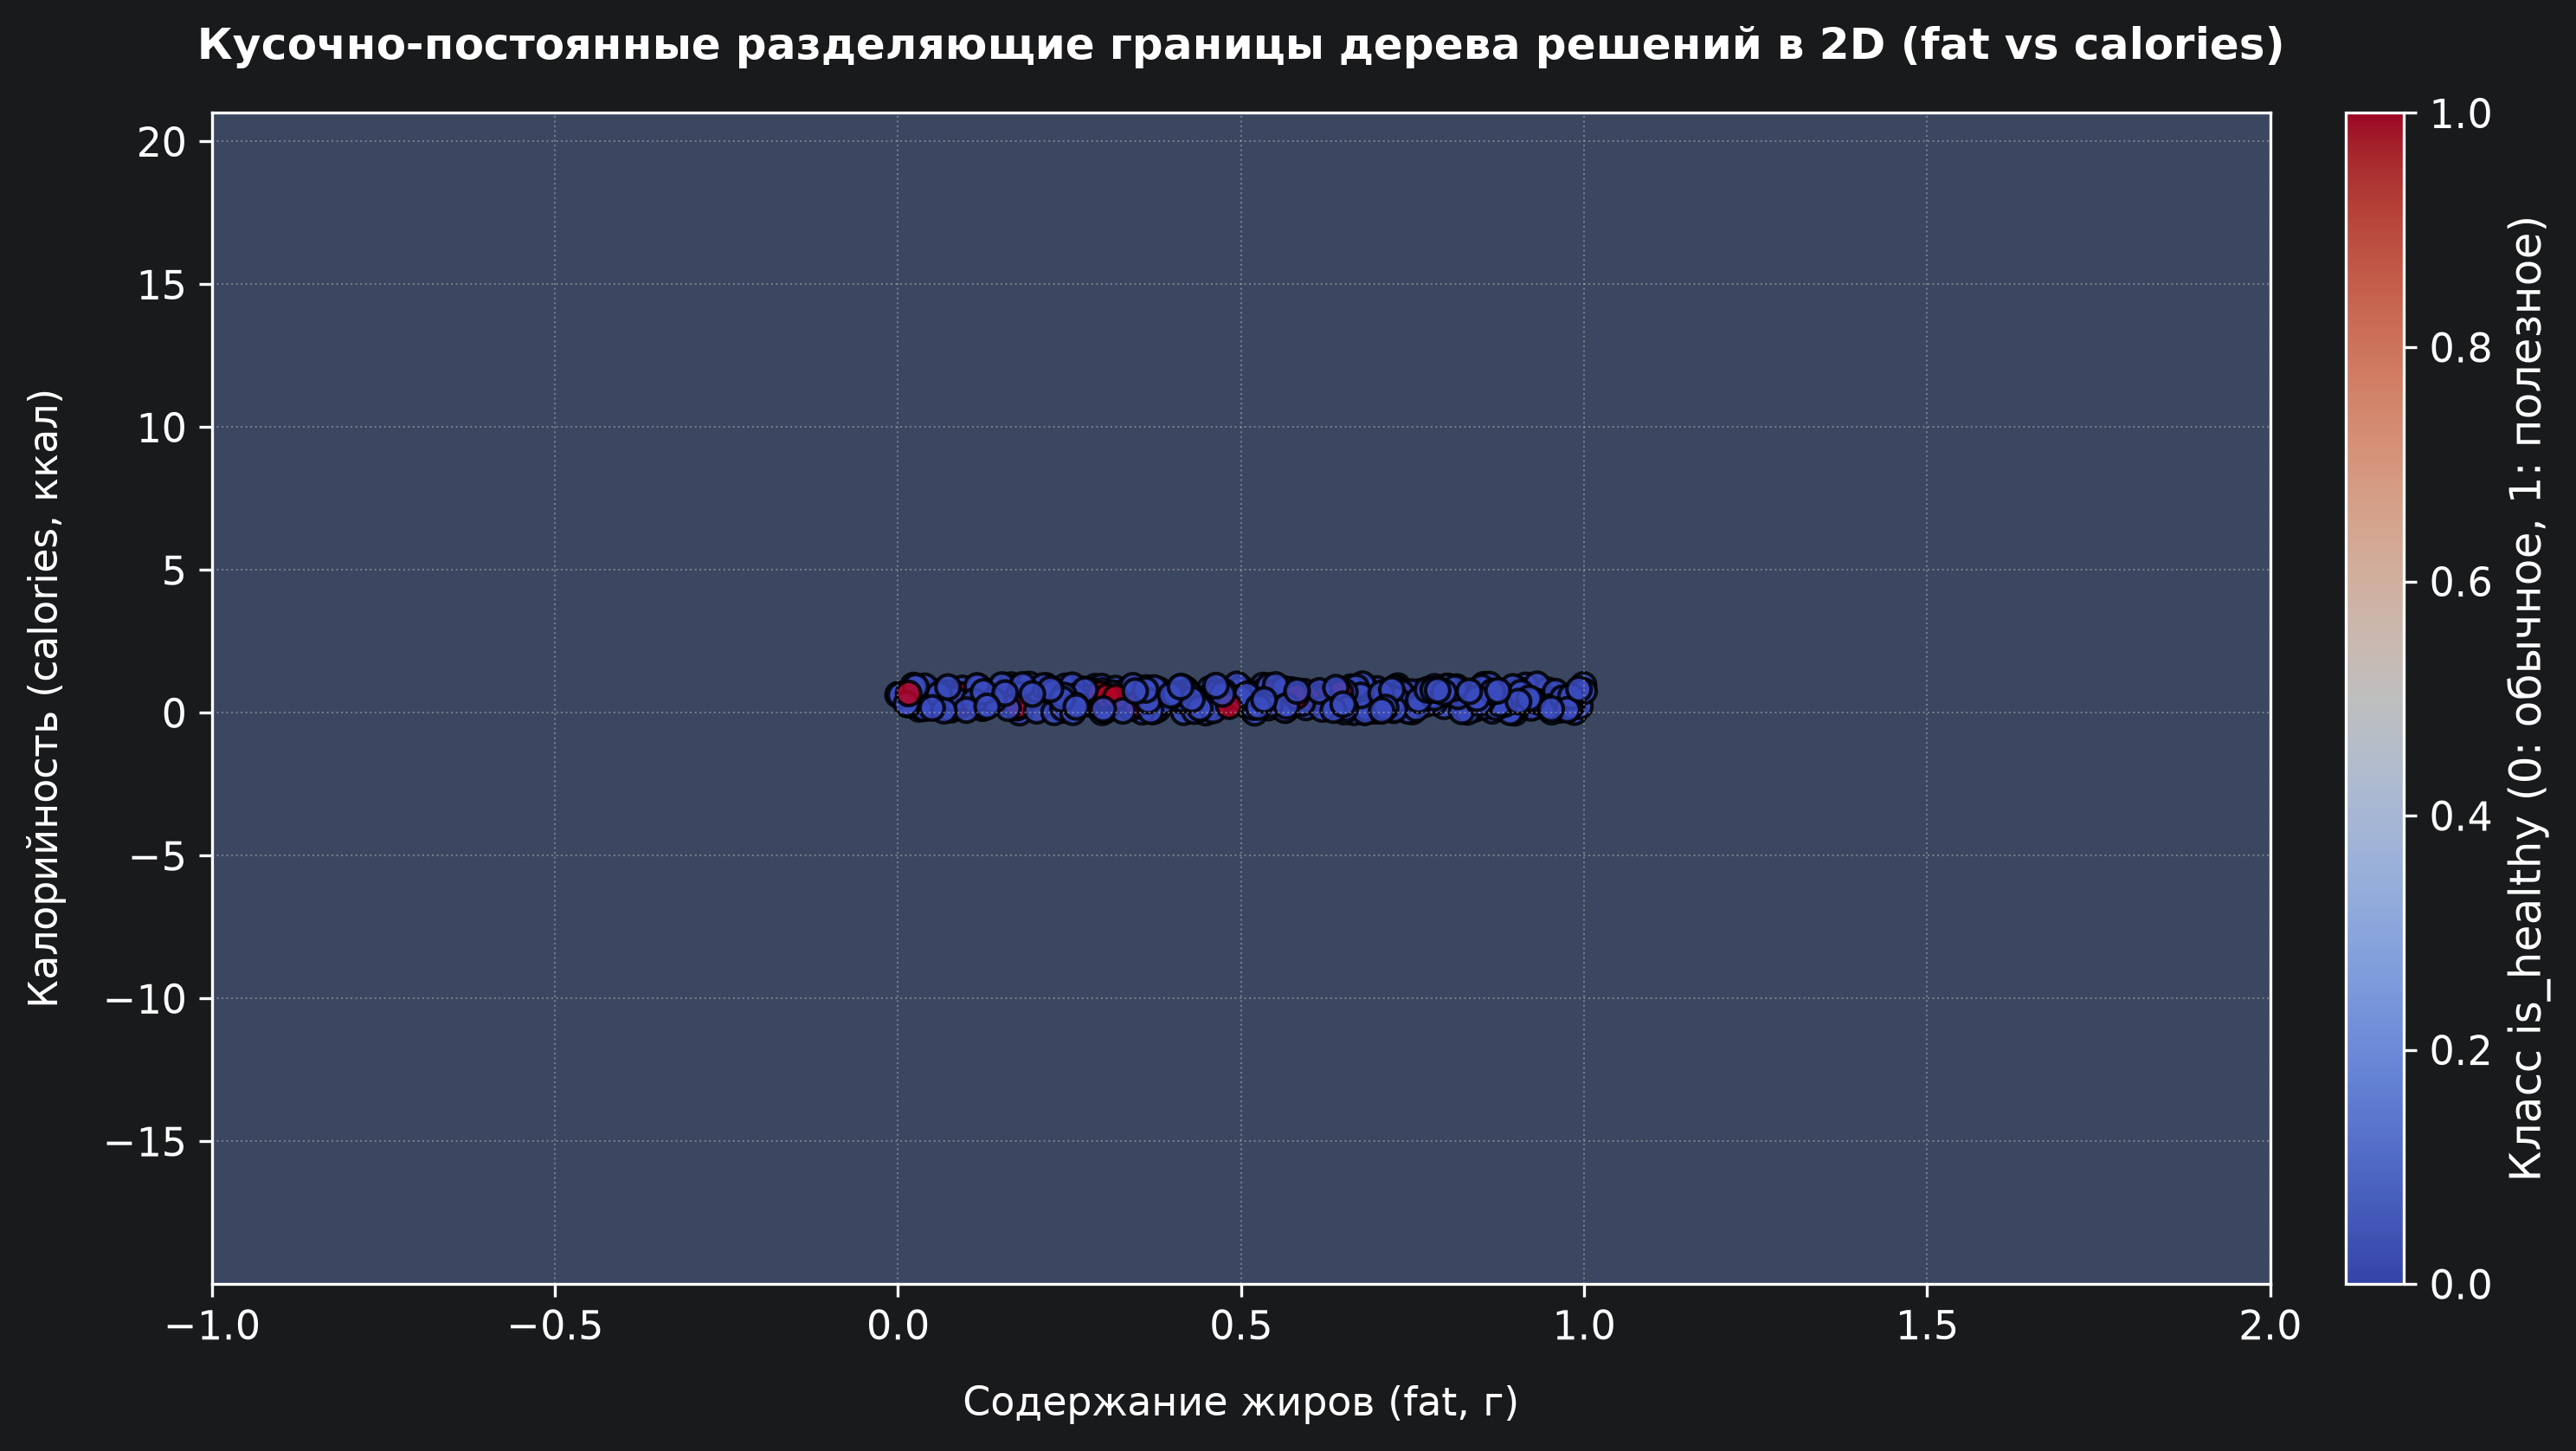
\includegraphics[width=0.88\textwidth]{images/fig7_decision_boundary.png}
    \caption{Кусочно-постоянные разделяющие границы решающего дерева в 2D-пространстве}
    \label{fig:decision_boundary}
\end{figure}

В таблице 1 сведены результаты верификации самописного классификатора с эталонной моделью \texttt{Scikit-Learn}.

\begin{table}[H]
    \caption{Сравнение самописного дерева и эталона Scikit-Learn}
    \label{tab:benchmark}
    \centering
    \small
    \begin{tabularx}{\textwidth}{lcccc}
        \toprule
        \textbf{Датасет} & \textbf{max\_depth} & \textbf{Custom Acc} & \textbf{Sklearn Acc} & \textbf{Совпадение, \%} \\
        \midrule
        make\_classification & 1 & 0.7733 & 0.7733 & 100.0\% \\
        make\_classification & 2 & 0.7733 & 0.7733 & 100.0\% \\
        make\_classification & 3 & 0.7867 & 0.7867 & 100.0\% \\
        make\_classification & 4 & 0.8000 & 0.8000 & 100.0\% \\
        Healthy Meal Plans & 1 & 0.9040 & 0.9040 & 100.0\% \\
        Healthy Meal Plans & 2 & 0.9040 & 0.9040 & 100.0\% \\
        Healthy Meal Plans & 3 & 0.9040 & 0.9040 & 100.0\% \\
        \bottomrule
    \end{tabularx}
\end{table}

% ==============================================================================
% 7. ВЫВОДЫ ПО ЛАБОРАТОРНОЙ РАБОТЕ
% ==============================================================================
\section{Выводы}

В ходе выполнения лабораторной работы:
\begin{enumerate}
    \item Изучен теоретический и математический фундамент построения решающих деревьев CART.
    \item С нуля на базовом Python и библиотеке \texttt{numpy} реализованы функции расчета критерия Джини ($Gini$), прироста информации ($Information\ Gain$), разбиения выборки, критериев останова и метрики $Accuracy$.
    \item Разработан классификатор \texttt{DecisionTreeClassifierCustom}, совместимый со стандартом Scikit-Learn (\texttt{fit}, \texttt{predict}, \texttt{score}).
    \item Исследовано влияние критериев останова: продемонстрировано, что неограниченное увеличение глубины ведет к переобучению ($overfitting$), в то время как ограничение глубины ($\texttt{max\_depth} = 3$) обеспечивает наилучшую обобщающую способность ($Accuracy = 90.4\%$).
    \item На синтетических данных \texttt{make\_classification} и реальном наборе \texttt{Healthy Meal Plan Dataset} доказано полное (100.0\%) совпадение результатов самописного дерева с эталонной моделью \texttt{sklearn.tree.DecisionTreeClassifier}.
\end{enumerate}

\end{document}
